\chapter{Design and Implementation}\label{ch:implementation}
In this chapter a preliminary test will present a study into users’ pleasure, arousal, and feel of control, as well as the average time that users are willing to spend when watching an AR overlay without interacting with it. The latter has been used as the estimation for a baseline for how much time a user can be expected to spend when just looking at an AR application. Following that section an overview of the design including a storyboard, UML diagrams of the system and user interaction\todo{do we need these? we haven't made them}, and the minimum implementation requirements needed to execute the evaluation. Next is described, both the tools used for the implementation and the implementation process from sketch to model are described accompanied by explanations to the implementation of the AR system. 

\section{Preliminary Interest Test}
For the purpose of testing different methods of data gathering for the evaluation a preliminary test was conducted. This test also served the purpose of obtaining a baseline for the length of time users might spend on an AR application, which also served as an answer to research question 1: \textit{When presented with an AR application with no features other than showing a model, for how long will users generally be willing to direct their attention towards the application?}


\subsection{Metrics}\label{subsec:premetrics}
For this test four different sets of data were gathered. Two of the metrics were self-reporting, meaning the participant chose the answer. The other two metrics were data gathered by the sensors attached to the arduino and to the participant. The four parameters are as follows:
\paragraph{Electrodermal activity (EDA):} The EDA sensors measure the skin conductance of the wearer. This is used to read the wearer’s level of arousal, which rise and fall depending on the task of the wearer and how exciting they find the task. The more aroused the wearer is, the more sweat will be generated and thereby increasing the conductance.
\paragraph{Inter-Beat interval (IBI):} The IBI sensor measures the heart rate variability (HRV) which varies from beat to beat, by recording the beats of the pulse. The more relaxed a person is the more variability there is between the beats, and vice versa. 
\paragraph{Time:} Throughout the experiment, the time is recorded. This was done by having the facilitator stop the timer when receiving a notice from the participant to stop, since the equipment work by the participant during the test prohibited them from stopping the timer themselves.
\paragraph{Self-assessment manikin (SAM):} As described by Bradley and Lang (1994), SAM is a picture-oriented instrument to assess a subject’s pleasure, arousal, and feeling of control in response to a stimulant. The three rows, seen in Figure \ref{fig:SAM}, each represent one of these parameters on a 5-point scale with graphic depictions \cite{Bradley1994}. Subjects may point at the image which best represents their feeling of pleasure, arousal, and control. SAM is a efficient useful tool for determining the participants reported experience of emotions associated with the presented stimuli. 

\begin{figure}[h!]
    \centering
    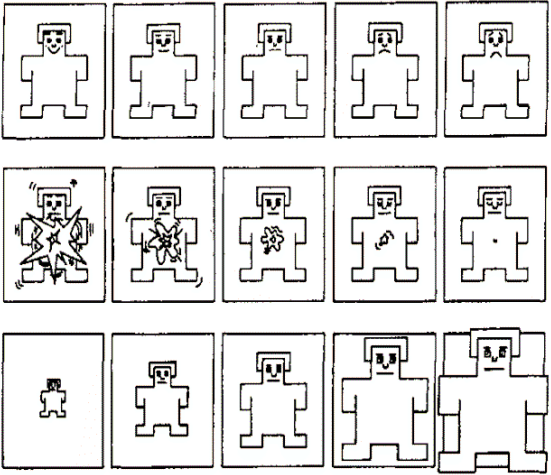
\includegraphics[width=\textwidth]{figures/SAM.png}
    \caption{The three SAM scales: Pleasure (top), arousal (middle), and control (bottom) \cite{Bradley1994}}\label{fig:SAM}
\end{figure}

\pagebreak

\subsection{Setup}
The following tools are used for the purposes of the preliminary interest test:

\begin{itemize}
    \item A smartphone with the AR application \textit{AR Dino Roar} installed
    \item An arduino with breadboard (as well as the necessary wires to connect everything)
    \item Two EDA sensors
    \item A pulse sensor
    \item A smartphone to serve as a stopwatch
    \item A computer to which the arduino is connected
    \item A camera to film the procedure
    \item A piece of paper with a pattern to serve as an AR marker
    \item A piece of paper showing the SAM scales
\end{itemize}

\textit{AR Dino Roar} is an application for android devices in which users may use their own pattern as an AR marker. The application then displays a model of a dinosaur in AR. A screenshot of this application can be seen in Figure \ref{fig:dino}. This application was chosen based on its similarities with the application being used for the final evaluation. It is a static 3D model that can be viewed from several angles, but does not have any other significant features. Therefore it was deemed appropriate for determining the average amount of time participants will look at an AR application with no outside context. 

\begin{figure}[h!]
	\centering
    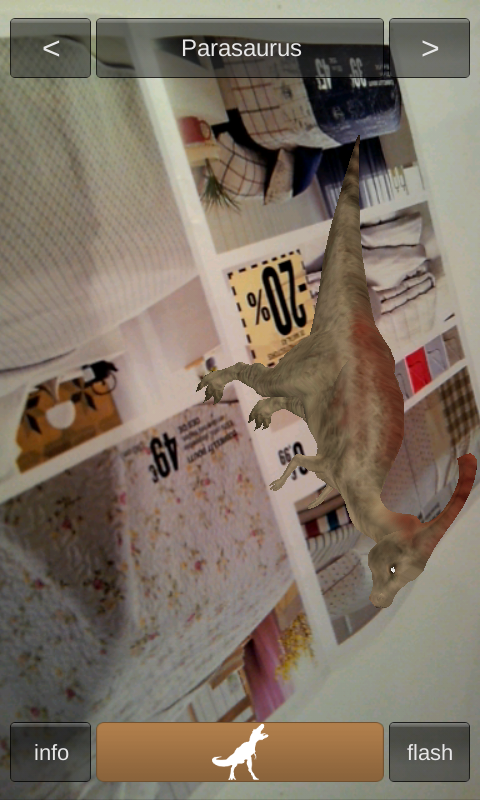
\includegraphics[scale=0.5]{figures/AR_dino.png}
    \caption{A screenshot of the AR Dino Roar app \cite{ARDino}}\label{fig:dino}
\end{figure}

In the test setup, a circuit is set up with the arduino, breadboard, sensors and wires in such a way that one can measure a participant’s EDA and IBI. The arduino is connected to the computer so that this data may be recorded. The EDA sensors are attached to the left index and middle finger of the participant, and the pulse sensor is attached to their left ear lobe, as seen in Figure \ref{fig:pretest_ear}.

\begin{figure}[h!]
    \centering
    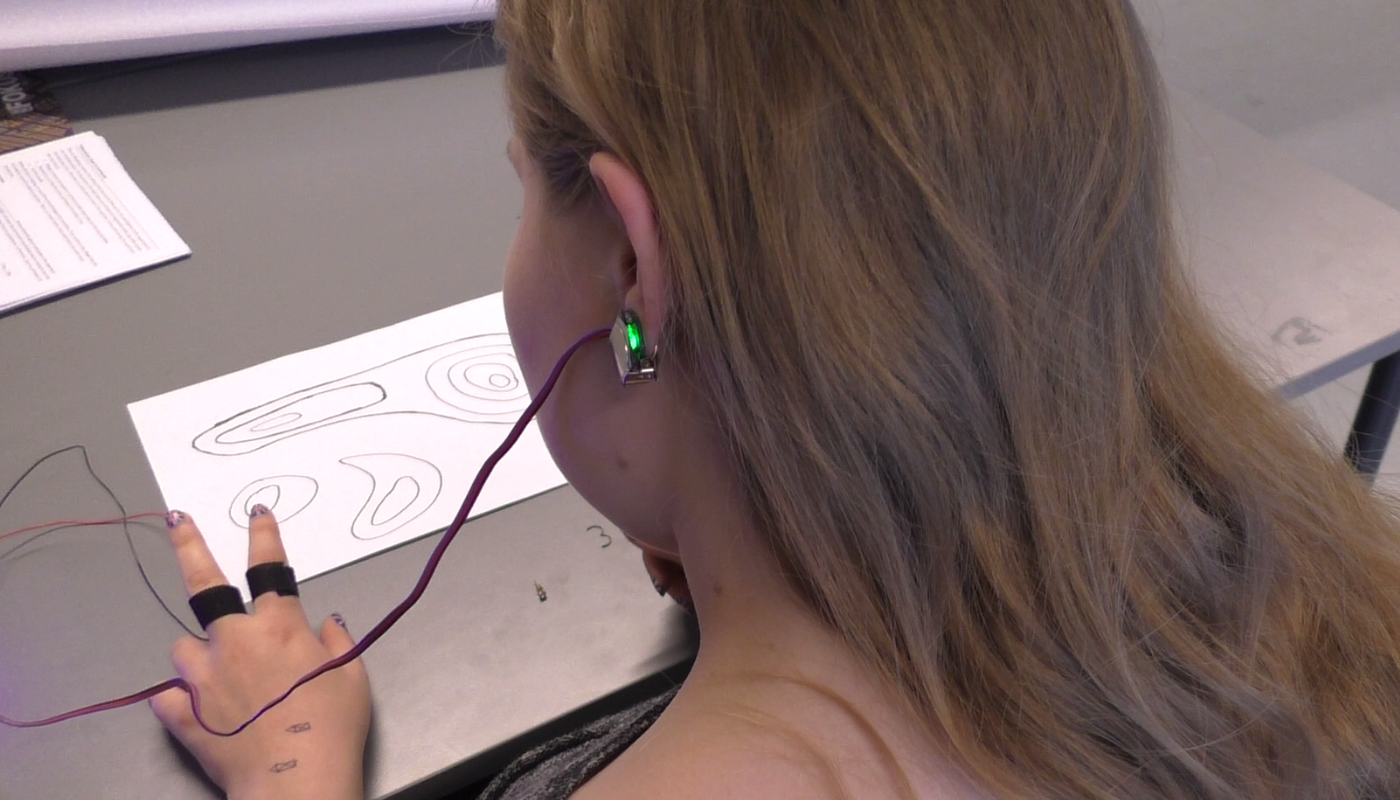
\includegraphics[width=0.8\textwidth]{figures/pretest_ear.png}
    \caption{The EDA and pulse sensors attached to a participant}\label{fig:pretest_ear}
\end{figure}

The test participant is seated in front of a table. On this table is the AR marker, the two smartphones, the SAM paper, and the arduino to which the participant is connected. The test facilitator is seated next to the participant in front of a computer, on which they record results from the test. The full test setup can be seen in Figure \ref{fig:pretest_setup}.

\begin{figure}[h!]
    \centering
    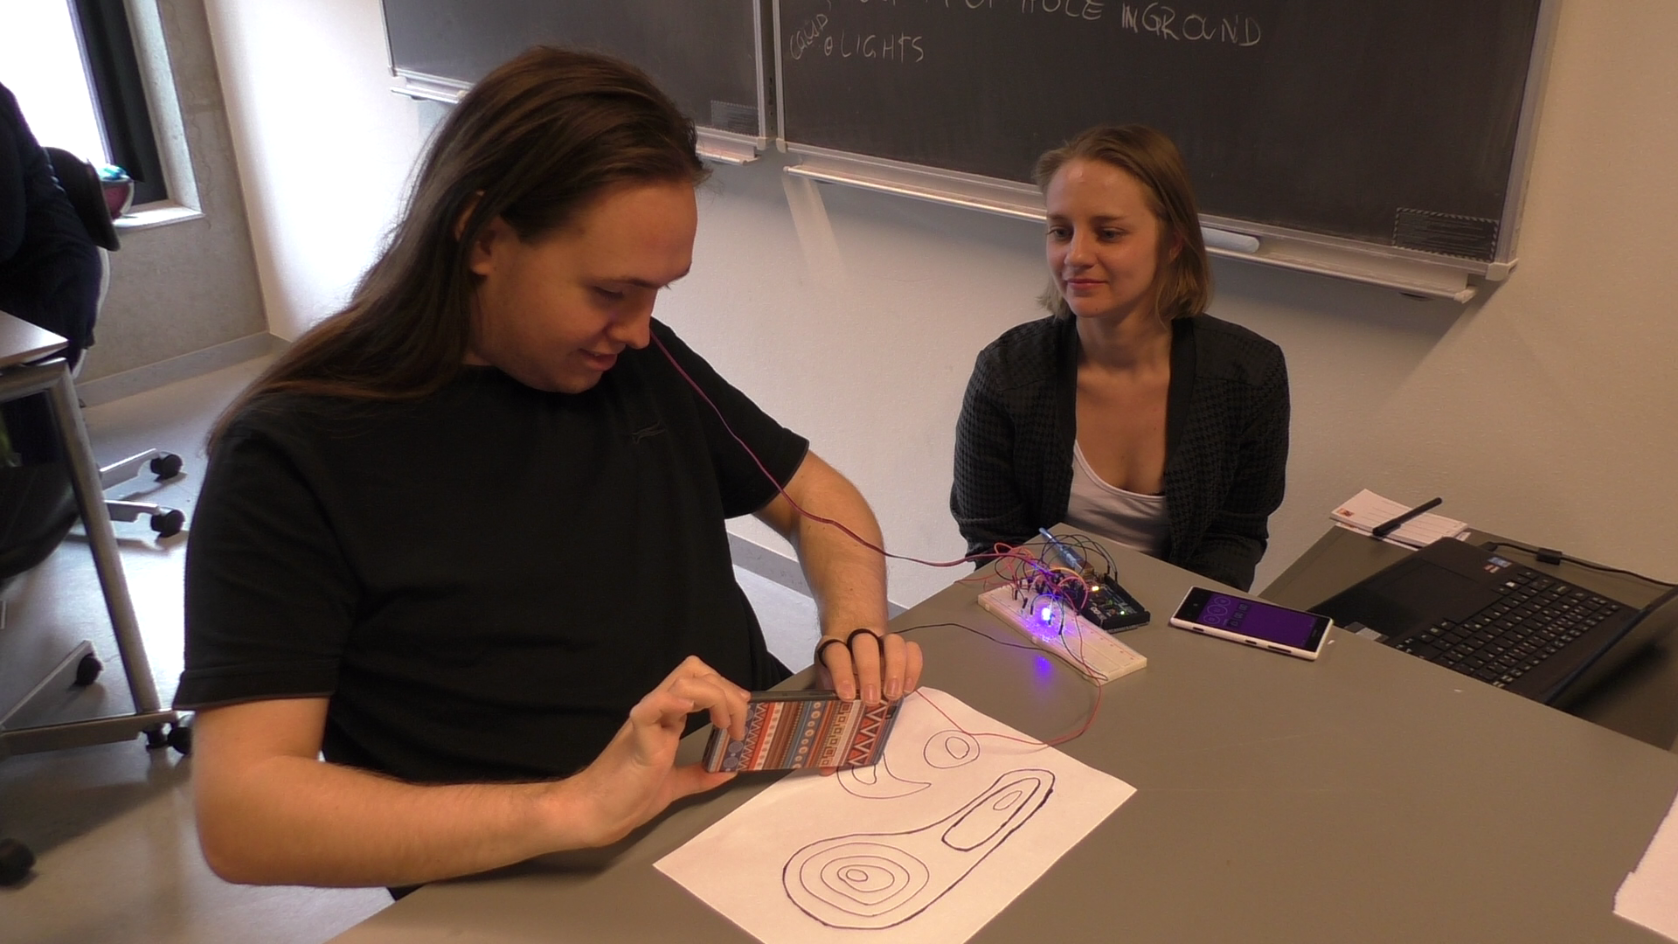
\includegraphics[width=0.8\textwidth]{figures/pretest_setup.png}
    \caption{The setup for the preliminary interest test}\label{fig:pretest_setup}
\end{figure}

\subsection{Procedure}
Before the test begins, the facilitator explains the procedure to the participant. They then attach the sensors to the participant as described in the previous section. Before the participant interacts with anything, they must sit idly for one minute, so that a baseline IBI and EDA may be recorded. They are then asked to use the AR Dino Roar app to look at a virtual dinosaur. The stopwatch is started once they begin, and they are asked to tell the facilitator to stop the timer once they are no longer interested in the app. Their IBI and EDA is recorded while they interact with the app. Once they are done interacting with the app, they are asked to answer three questions using the SAM diagram: how pleased, aroused, and in control they felt, respectively. For each question, they were asked to point to one of five images in a given row which best described their feelings, as described in section \ref{subsec:premetrics}.

\subsection{Analysis of results}
Out of the ten tests only seven sets of data were usable in regards to the logging of the sensor data. At some point after test number 5, an error occurred within the arduino circuit, likely loose wires which affected the data gathering. This means that only seven sets of data from the EDA and IBI sensors are useful, which is not enough to make a clear conclusion on arousal or HRV. The graphs, seen in appendix \ref{ch:appA}, are all very stable.

The average time participants spent on the app is 52.20 seconds. However, the data gathered from the timer comes with two outliers caused by unintended interaction with the app and technical issues respectively. These outliers have a considerably impact on the average time, which when leaving out the outliers comes down to 37.75 seconds. 

The pictures in each row of the SAM sheet are labeled 1 through five, so that 1 corresponds to most pleased, most aroused, and least in control, and 5 corresponds to least pleased, least aroused, and most in control. This makes it possible to find the median of each scale. The median response for level of pleasure is 2, which is the slightly pleased manikin. The median response for arousal is 4, which is the second-least aroused manikin. The median response for control is 2.5, meaning that the median falls between the second-least in control and the neutral manikin. It is possible that the low level of arousal and control is caused by the low level of interactivity to the app, as there is little to do but look at a static AR projection of a dinosaur. Despite the low ratings of these aspects, test participants felt slightly more pleasure than neutral. 

\subsection{Discussion}
The primary purpose of this test was to learn how long a user will spend on an AR application with no features other than showing a model. The test only had 10 participants, which is not an adequate number to base a conclusion on, but it is adequate to describe a tendency or to establish a baseline for further testing. Out of the four different metrics measured, only two were useful for this purpose because of the faulty data. 

One was measuring the amount of time they used the app until they stated that they were no longer interested. The average for this test was 52.20 seconds, however removing two outliers reduced it to an average of 37.75 seconds. This can be used as a baseline for how long we expect the participants to use the app during the evaluation.

Additionally, the SAM gave useful information. The parameters allow users to articulate through images how their experience was. A similar inquiry may be made in the final evaluation of this project. A factor to consider with all three SAM scales is the context of usage. For this test, the participants had no outside context to use the application (such as a tour guide explaining material which is relevant to what can be seen on the screen), and this might have affected the overall experience. 

The EDA and IBI data was very inconclusive, and due to technical difficulties only a bit more than half of the data was valid. This means that it would be inappropriate to use it for the final evaluation, especially since it would also be cumbersome and resource-heavy to bring it for the evaluation which will not be stationary and moreover takes place outside with several participants at a time.

\section{Minimum Implementation Requirements}
To define the minimum implementation requirements by priority the MoSCoW method developed by Dai Clegg \todo{\cite{Kuhn}} is used to sort the various features for the concept. MoSCow in itself is an acronym which is derived from the first letter of each priority category (Must have, Should have, Could have, and Won’t have but would like). Listed the MoSCoW priorities read as follows:

\textbf{Must have}:
\begin{itemize}
\item A 3D model placed such that it seems to be a hole in the ground when projected onto an image of the street
\item Ability to read a marker and project a 3D model onto it
\end{itemize}

\textbf{Should have}:
\begin{itemize}
\item Shaders and textures for the 3D model to make it look like a dungeon
\item Appropriate light setting
\item Details to the model such as a staircase and chains
\item The model should be angled in such a way that its perspective lines up with the images captured by the camera
\end{itemize}

\textbf{Could have}:
\begin{itemize}
\item Additional details to the model, such as a prisoner, straw, dirt etc.
\item Realistic looking light based on predictable information
\end{itemize}

\textbf{Won’t have but would like}:
\begin{itemize}
\item Markerless detecting system
\item Light adjustment system that adapts to weather type and time of day
\end{itemize}

It is found to be of the utmost importance to have a basic 3D model of the subterranean site. Further it is paramount for the users to be able to project this model onto their smartphone screen by registering a marker of some sort. The reasoning behind this priority is that the project first and foremost is about showcasing non-visible scenes occurring on a guided tour and see if this impacts the user experience, cf. the problem statement. 

It has also been deemed to be of some importance to have the model equipped with appropriate shaders and textures lit by a proper set of light sources. As it is explained in the previous chapter, a research study found that textures and shading in accordance with the light improves the 3D percept. Alongside, the texture in relation to the light choices should emphasise the atmosphere of a dungeon. Therefore some explanatory additions to detail the purpose and context of the model should be added e.g. stairs to state it to be on the lowest level (basement level), and chains to indicate prison. 

Of less importance is considerations to a realistic light setting in accordance with the predictable environmentals (e.g. existing buildings and sun orientation at a specific time of day) as well as higher levels of details to the model. Although details like piles of straw, dirt, prisoners, etc. could potentially improve the emphasis to the model and its contents, it is not part of the project’s main objective. Also despite having a light adjusting system which adapts to different weather conditions and time of day would be a nice addition which could add on to the realism of the scene, this has been considered out of the project scope. Lastly, though a markerless system would be a practical part of the finished application since this would make it easier for the guide to manage the application compared to bringing markers along, for the test purpose such a system has been found unnecessary to implement.


\section{Implementation}
For the purpose of creating the 3D model, the 3D model program Autodesk Maya has been used. The model is based on sketches of the site, as will be explained in the following sections. For creating the application itself, the Vuforia plugin for Unity has been used. The marker consists of an image printed on two A3-sized sheets of paper, which have been attached to a piece of cardboard in order to make the marker more stiff. \todo{probably needs references for the different programs}

\subsection{From Sketch to Model}
\begin{wrapfigure}{r}{0.35\textwidth}
\centering
        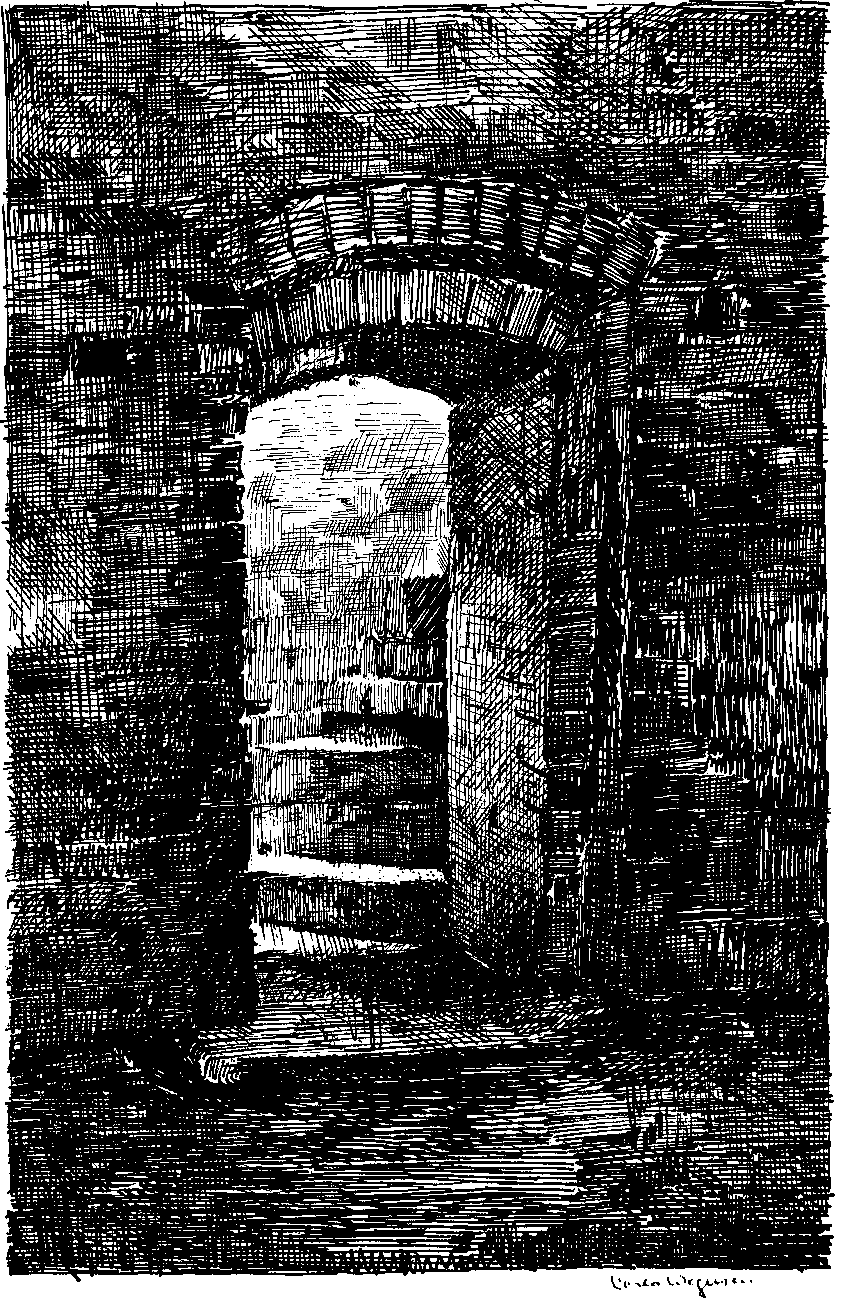
\includegraphics[width=0.3\textwidth]{figures/sketch1.png}
        \caption{Illustration by Carlo Wognsen of the dungeon beneath Vesterport, south wall with access to spiral staircase leading up to street level \cite{Riismoller1961}}\label{fig:sketch1}
\end{wrapfigure}

In order for the 3D model to be representative to the real “Rakkerens Hule”, the dimensioning and shape is primarily inspired by the architectonic sketches made of the excavated ruins of the prison at the western city gate of old Aalborg after its rediscovery in 1907. These were prepared by architect H. Paludan at the request of Nationalmuseet, see Figure \ref{fig:sketch0}. Another source is the descriptions of the site by Chr. Axel Jensen from 1909 \cite{Jensen1909}. Inspiration has also been drawn from the illustration of the south wall made by Carl Wognsen \cite{Riismoller1961}, seen in Figure \ref{fig:sketch1}.

\begin{figure}
    \centering
    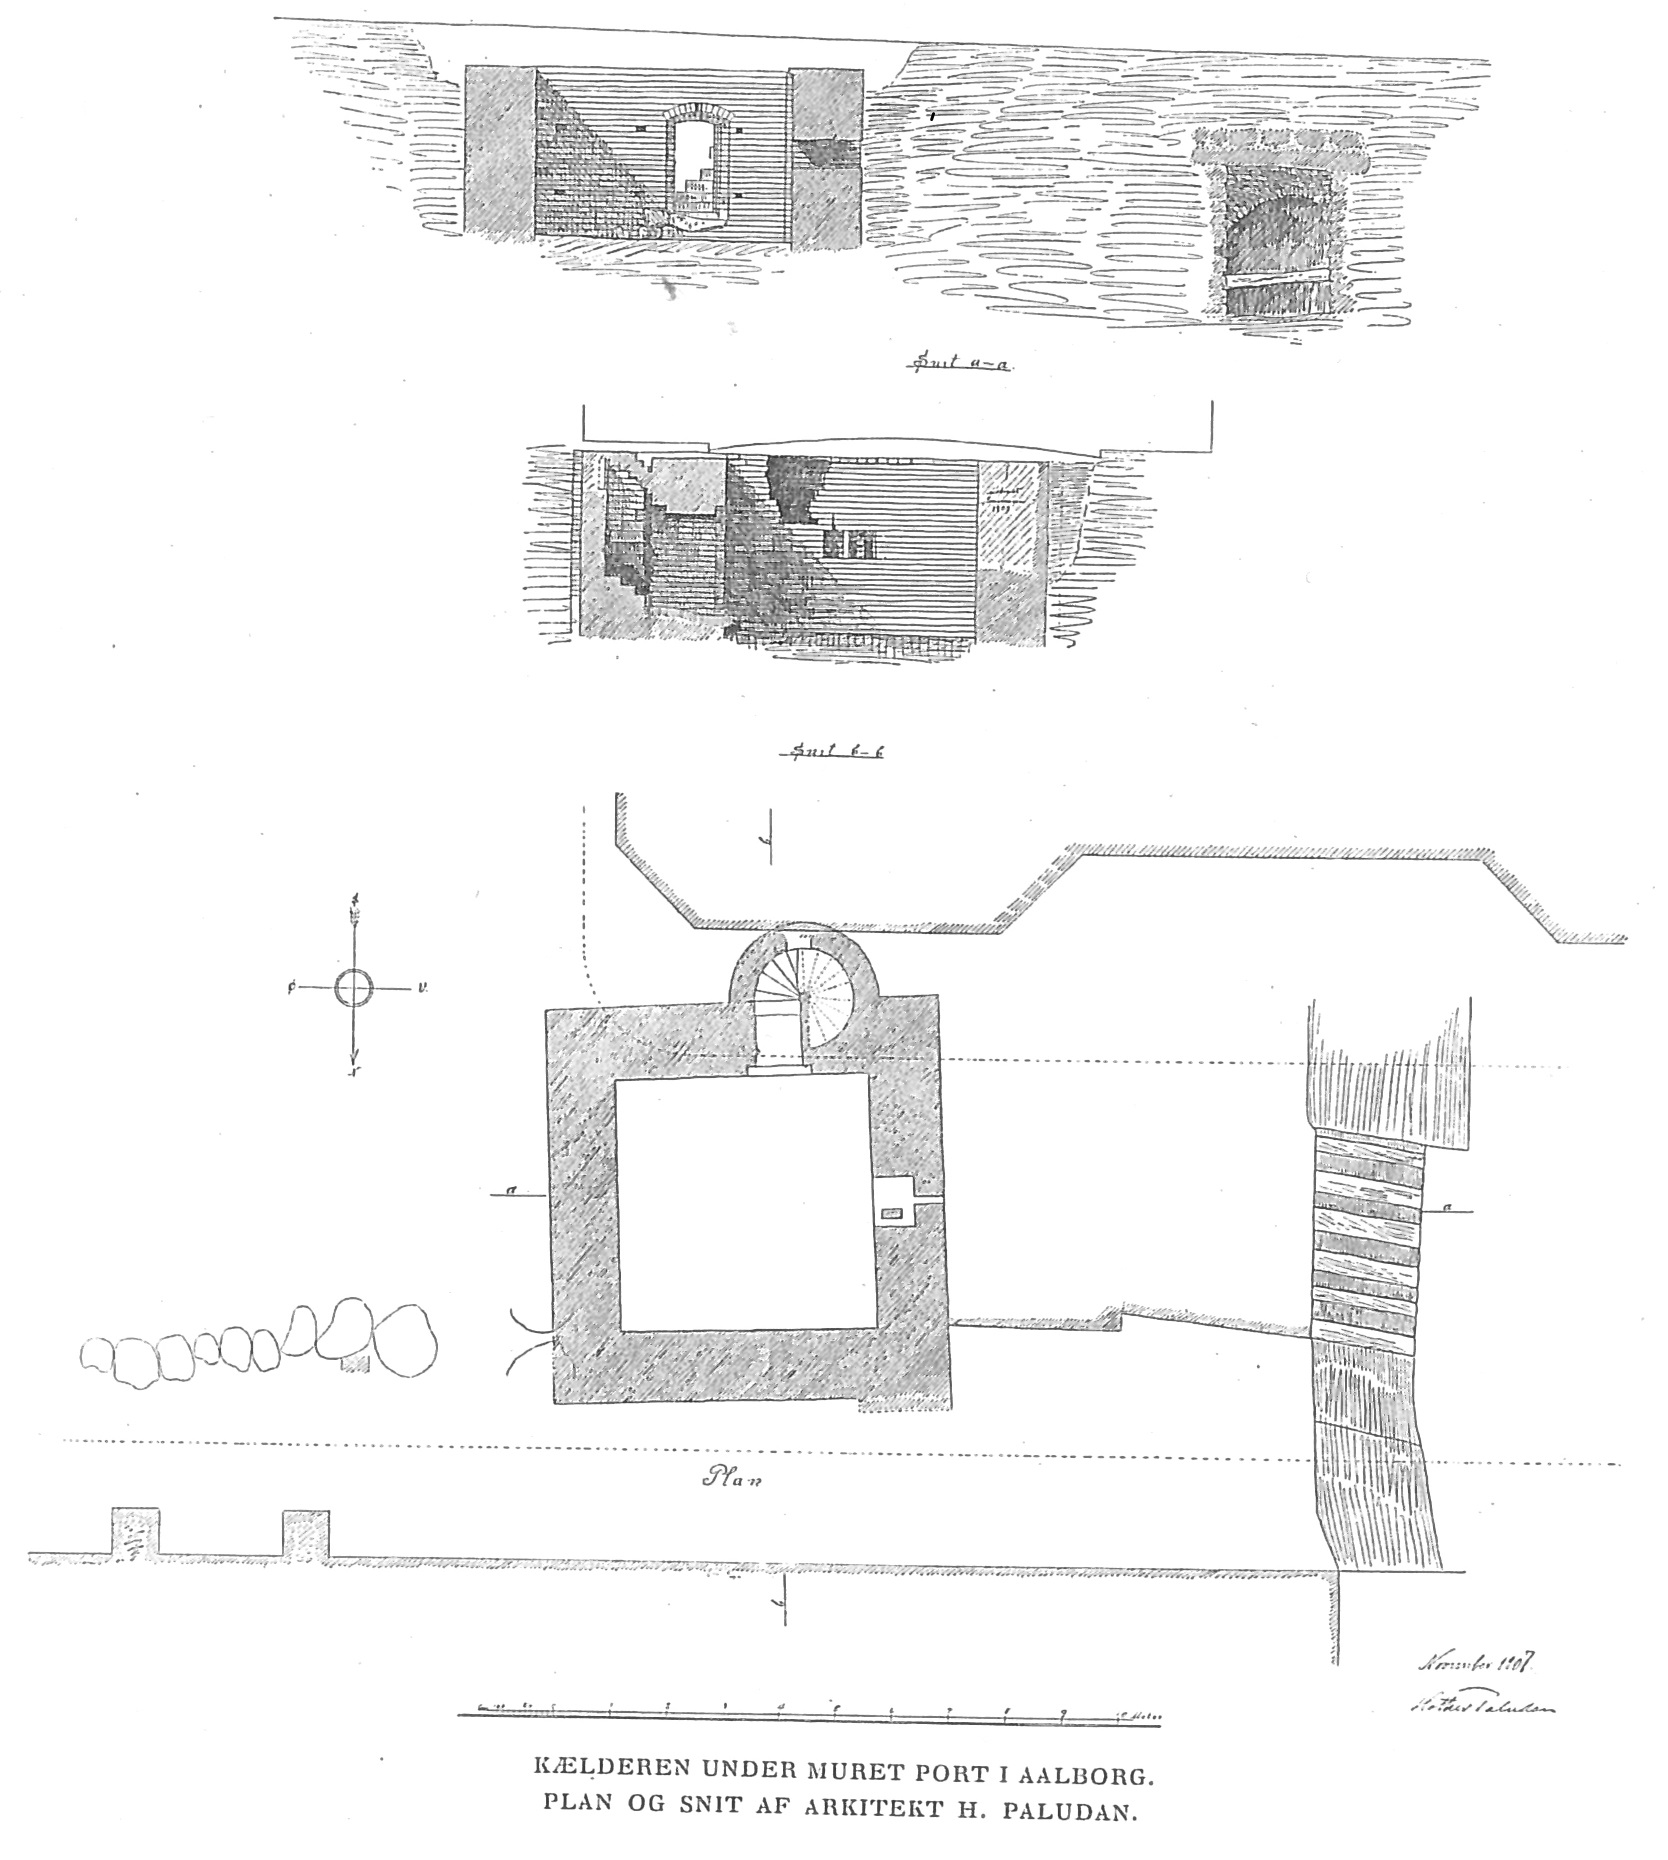
\includegraphics[width=\textwidth]{figures/sketch0.jpg}
	\caption{The dungeon beneath Vesterport in Aalborg, plan and section by architect H. Paludan \cite{Jensen1909}}\label{fig:sketch0}
\end{figure}

\begin{figure}
    \centering
        \begin{subfigure}[h!]{0.7\textwidth}
    	\centering
        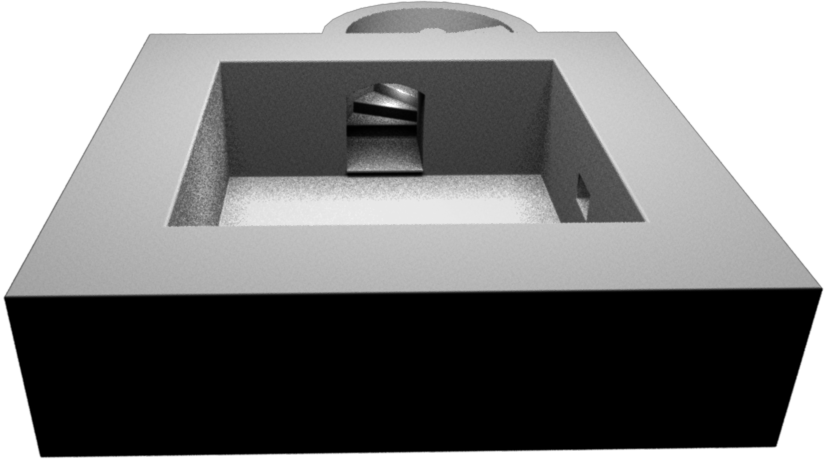
\includegraphics[width=\textwidth]{figures/model.png}
        \caption{The model of the dungeon, untextured}\label{fig:model}
    \end{subfigure}
    \begin{subfigure}[h!]{0.7\textwidth}
    	\centering
        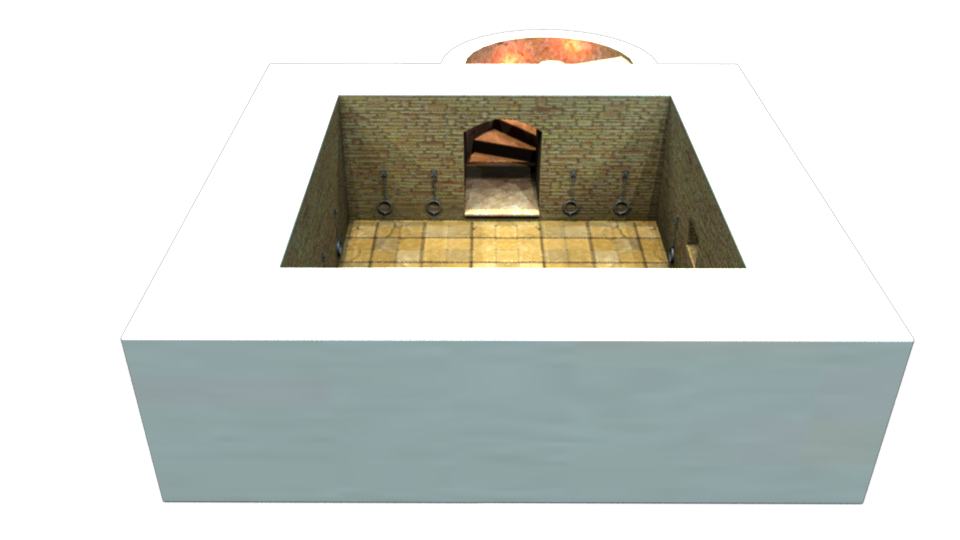
\includegraphics[width=\textwidth]{figures/model_total.png}
        \caption{The full model, with textures}\label{fig:total}
    \end{subfigure}
    \begin{subfigure}[h!]{0.7\textwidth}
    	\centering
        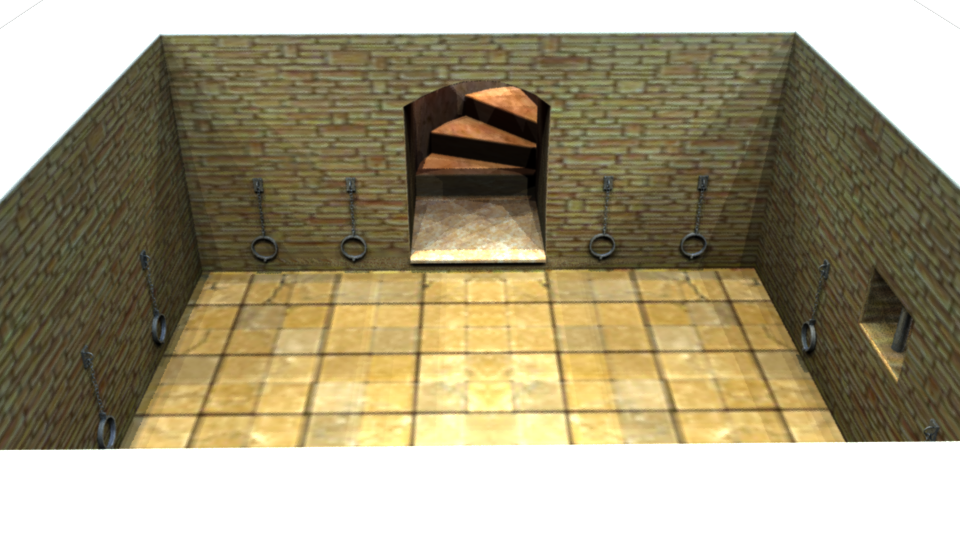
\includegraphics[width=\textwidth]{figures/model_long.png}
        \caption{The model as it will approximately look in the app}\label{fig:long}
    \end{subfigure}
    \caption{The model of \textit{Rakkerens Hule} to be used in the application}
\end{figure}

The base shape of the 3D model made from the sketches can be seen in Figure \ref{fig:model}. It is made of the geometric primitives: cube, cylinder, and pipe. The cube is used for the floor from which the walls and the staircase have been extruded, whereas the holes for the doorway and embrasure result from bridging the edges, left after the removal of strategic wall faces. A cylinder is used to make the bar in the prison window and the spindle directing the winding staircase. Lastly, half a pipe has been used to make the walls surrounding the staircase.%\pagebreak

Aside from the descriptions and sketches of the prison’s structure another source was found Jørgensen \cite{Jorgensen1934} and Jensen \cite{Jensen1909} which provided the description of the building materials for the prison. For instance they describe how the prison walls were constructed out of yellow bricks, the floor in the doorway consisted of granite, and the outside walls were covered with a layer of lime mixture. Images of the model with its textures can be seen in Figure \ref{fig:total} and \ref{fig:long}.

\begin{wrapfigure}{l}{0.2\textwidth}
   \centering
   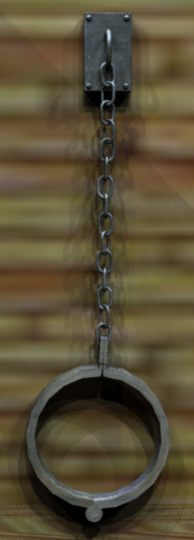
\includegraphics[width=0.18\textwidth]{figures/chainmodel.png}
   \caption{Close-up of a chain from the dungeon model}\label{fig:chain_model}
\end{wrapfigure}

Like the prison itself, the models of the chains is based on the design of real chains from the renaissance period found during archeological excavations, sketched by Carl Wognsen \cite{Riismoller1961}, see Figure \ref{fig:chains}. Primarily the illustration of the neck iron (Figure \ref{fig:chains1}) has been used since only the neck iron is meant to be attached to a wall in the dungeon. However, the chain part of the handcuffs has inspired the design of the chain device connecting the neck iron to the prison wall.

\begin{figure}
    \centering
    \begin{subfigure}[h!]{0.3\textwidth}
        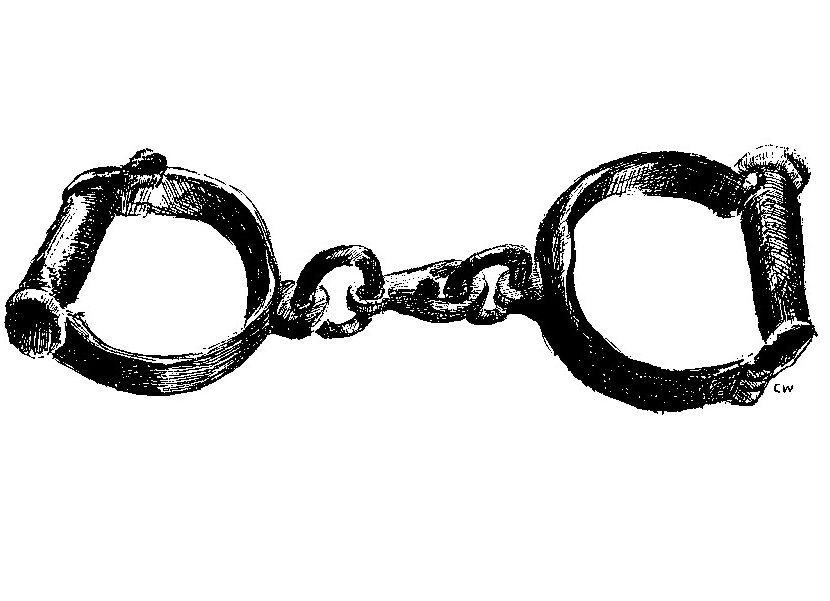
\includegraphics[width=\textwidth]{figures/chains0.jpg}
        \caption{Full illustration of handcuffs}\label{fig:chains0}
    \end{subfigure}
    \hfill
    \begin{subfigure}[h!]{0.3\textwidth}
        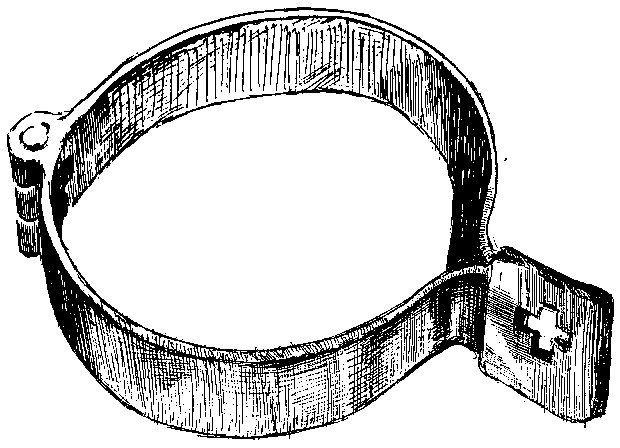
\includegraphics[width=\textwidth]{figures/chains1.jpg}
        \caption{Neck iron from the renaissance period. The cross shaped hole is for the chain}\label{fig:chains1}
    \end{subfigure}
    \hfill
    \begin{subfigure}[h!]{0.3\textwidth}
        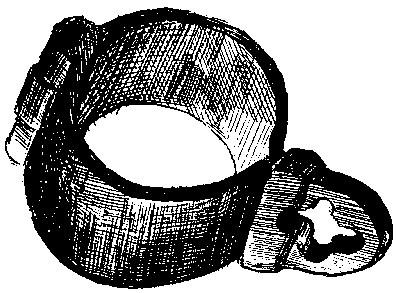
\includegraphics[width=\textwidth]{figures/chains2.jpg}
        \caption{Foot shackle from the renaissance period}\label{fig:chains2}
    \end{subfigure}
    \caption{Handcuffs from the town hall basement. Similar handcuffs may have been used in the dungeon. Illustration by Carlo Wognsen \cite{Riismoller1961}}\label{fig:chains}
\end{figure}

The 3D model is constructed from the primitives: pipe, cube, sphere, cylinder, and torus, textured with an iron texture, and it can be seen in its finalised version in  Figure \ref{fig:chain_model}. 
Two pipes and a cylinder make up the neck iron. Here one large pipe added some extrusions and bridges forms the main part. Meanwhile, does the other smaller pipe together with the cylinder compose the hinge (located at the bottom in the figure). Last but not least is the wall attachment made of a cube, four spheres cut in half as the screws and a round torus from which toruses prolonged into a chain joint shape is put in series in order to become the chain that connects the wall attachment with the neck iron.

\subsection{Light Sources}
The light setting consist of directional lights, three point lights, a spotlight, and an area light. To have the model’s entirety lit up as if situated outdoor on an average Danish spring day \cite{DMI}, a directional light with a faint tone of warm yellow has been utilised to emit the sunlight. More directional light sources with pale bluish tones have further been added to imitate the scattering of sunlight by atmospheric molecules in the sky --- a phenomenon also called Rayleigh scattering or critical opalescence \cite{DOE} \cite{Renn2005}. For the lighting of the staircase section a spotlight is used. Additionally, the staircase is lit up by three point lights with a deep orange tone to emulate torches hanging on the curved wall which can be seen in Figure \ref{fig:interior0}. Finally, an area light has been used to cast the light deriving from the embrasure hole, see Figure \ref{fig:interior1}.

\begin{figure}[h!]
    \centering
    \begin{subfigure}[h!]{0.8\textwidth}
    	\centering
        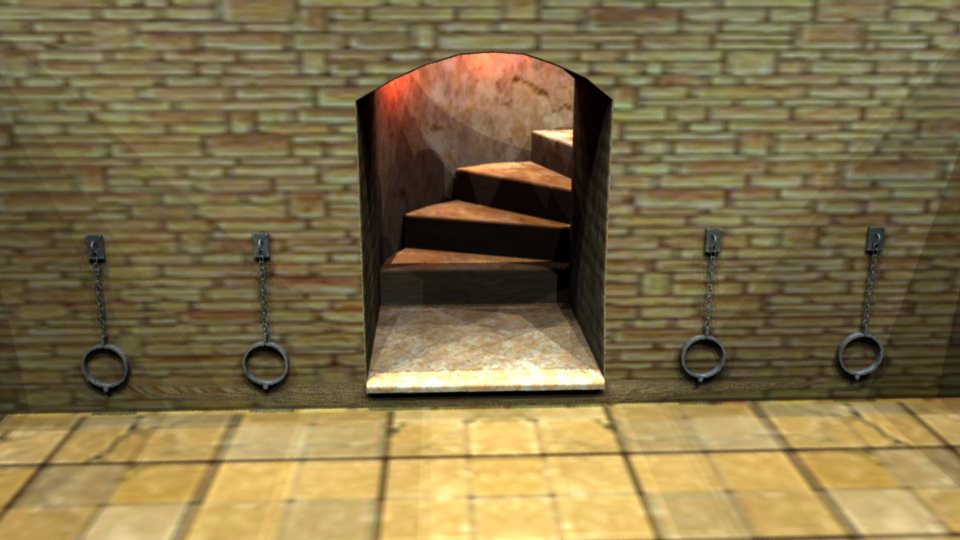
\includegraphics[width=\textwidth]{figures/interior0.png}
        \caption{The door in the dungeon, with visible staircase}\label{fig:interior0}
    \end{subfigure}
    \begin{subfigure}[h!]{0.8\textwidth}
    	\centering
        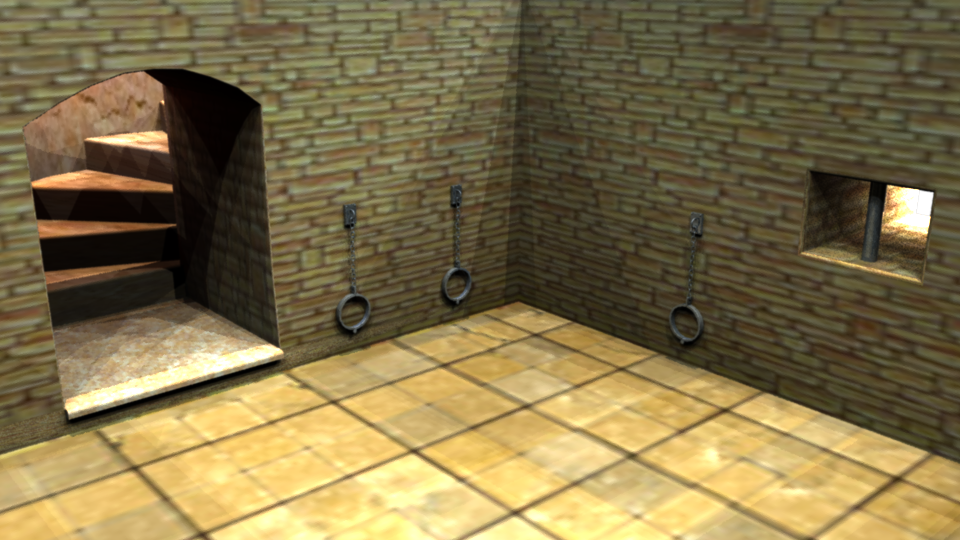
\includegraphics[width=\textwidth]{figures/interior1.png}
        \caption{The door, chains and window in the dungeon}\label{fig:interior1}
    \end{subfigure}
    \caption{Close-up of the interior of the model}\label{interior}
\end{figure}


\section{Implementation} \todo{all the citations in this section need to be implemented. sources are linked in the google doc called 'implementation part'} 
The project was developed in Unity \cite{unity_main_page}. In order to implement the design solution described in Section …\ref{sec:Design}, several methods were utilized. In general, the implementation of the design solution can be split into three parts: 
\begin{itemize}
\item Implementing AR
\item Making the illusion of seeing the 3D model through a hole in the ground
\item Adjusting lighting
\end{itemize}
Below, each of these three parts are described in detail. 

\subsection{Implementing AR}
In order to implement the AR part of the solution, an AR platform called Vuforia was used  \cite{Vuforia_main_page}. It is a marker based solution, where a marker can be a 2D image or a 3D object. For the purpose of this project, a 2D image was utilized. Unfortunately, since Vuforia is a commercial product, it is impossible to describe how exactly it is working. However, keeping in mind the background research described in Section …, it can be assumed that the software recognizes and tracks the marker, calculates its location in relation to the viewer, and places the 3D object accordingly. 

As it can be seen from the platform anatomy in Figure\ref{fig:imp1}, one way to create a marker in Vuforia is to load a JPEG or PNG image that will be transformed by the Target Manager into an Image Target. 

\begin{figure}[h!]
    \centering
    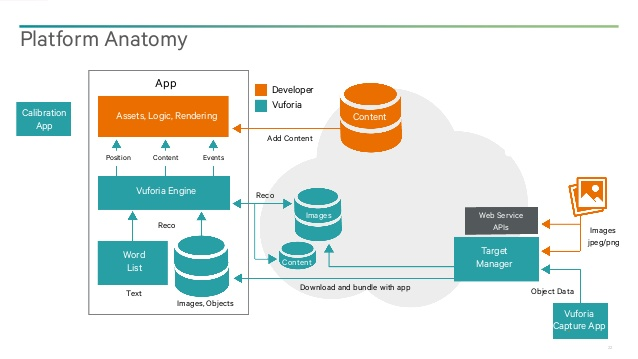
\includegraphics[width=0.8\textwidth]{figures/imp1.jpg}
    \caption{Vuforia platform anatomy}\label{fig:imp1}
\end{figure}


How well the software will  work is, in part, determined by the quality of the uploaded image. The quality of an Image Target is dependant on how many features an image has and how evenly those features are spread throughout the image. A feature is defined as a sharp angle of an edge extracted from the image \cite{Natural_features}. Therefore, for the purpose of this project, it was decided to use one image target with a lot of text over white background. The image that was used for the evaluation of our product can be seen in Figure \ref{fig:imp2}. 

\begin{figure}[h!]
    \centering
    
\includegraphics[width=0.8\textwidth]{figures/imp2.png}
    \caption{Image used for the evaluation marker.}\label{fig:imp2}
\end{figure}

The image was approximately 60 cm wide, which means that the image would have been recognized by the software up to a distance of about six meters \cite{calculate_distance_from_image}. Such a large image was used deliberately for two reasons. Firstly, the image had to be placed on the ground with participants standing around it and looking at it through their phones. This meant that if a participant was standing right next to the image, the distance between the phone and the image would have been approximately 1.5 meters. Secondly, the application was utilized as part of a guided tour experience with approximately ten people in a group. This meant that the participants would probably look at the image through their phones at a distance, forming a circle around the image, thus allowing for everyone to look at the image simultaneously. Having all this in mind and using the Pythagorean theorem, it could be calculated that a participant could stand as far as 5.8 meters from the image, and the phone could still detect it, as can be seen from Figure \ref{fig:imp3}. By using such a large image it was also possible to track it even if parts of it could not be seen. 
\begin{figure}[h!]
    \centering
    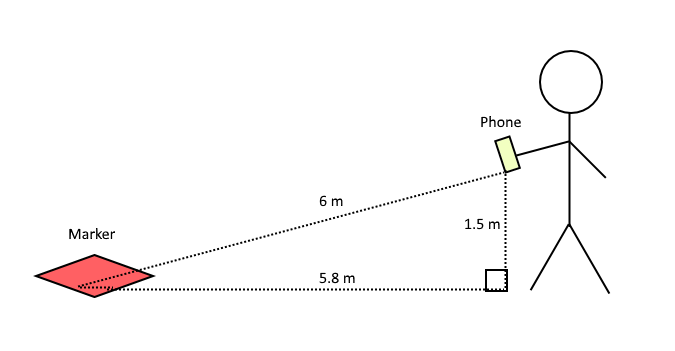
\includegraphics[width=0.8\textwidth]{figures/imp3.png}
    \caption{An approximate calculation of the maximum distance from the phone to the marker that can be reached without disrupting the detection of the marker.}\label{fig:imp3}
\end{figure}

\subsection{Making the illusion of a hole in the ground}
To make the illusion of a hole in the ground, the 3D model was placed right below the Image Target. It was also made transparent by using a material with a built-in shader from the Transparent shader family \cite{unity_legacy_shaders}.

Besides that, a plane was made in the shape and form of the hole through which the participants would view the 3D model. A material with a custom shader was applied to it. The shader resembles the Unity Standard Shader \cite{unity_standard_shader} with  a few extra lines added to it, which can be seen in Figure \ref{fig:imp4}. The first line, Zwrite Off, is responsible for not writing the pixels of the plane into the depth buffer, and ColorMask 0 checks that none of the plane pixels are rendered to any color channels. Thus, the plane is made transparent. Next, a stencil buffer is used to keep the pixels of the 3D model that are visible through the hole. The rest are discarded \cite{stencil_buffer}. Lines 6 and 8 ensure that a value of one would be written to the buffer. This means that a reference value of one would be assigned to those pixels that can be seen by the viewer through the hole. Comp always indicates that a stencil test will always pass. 

\begin{figure}[h!]
    \centering
    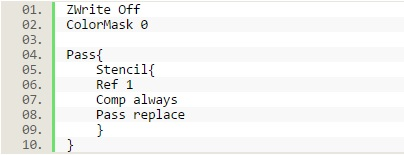
\includegraphics[width=0.8\textwidth]{figures/imp4.jpg}
    \caption{Extra code for the hole.}\label{fig:imp4}
\end{figure}

Similarly, a shader was applied to all of the materials of the 3D model. It also resembles the Unity Standard Shader with several lines added to it, which can be seen in Figure \ref{fig:imp5}. The code ensures that only the pixels with a reference value of one would be rendered.

\begin{figure}[h!]
    \centering
    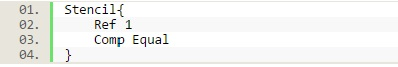
\includegraphics[width=0.8\textwidth]{figures/imp5.jpg}
    \caption{Extra code for the 3D model.}\label{fig:imp5}
\end{figure}

Furthermore, a 3D edge around the hole was made to make it more clear for the participants that they were looking through a virtual hole in the ground.

\subsection{Lighting}
The lighting of the model from Maya was unfortunately not able to be imported into Unity. Instead a minimum light solution was implemented, consisting of a directional light and a skydome. The shadows were disabled, leaving only the diffuse reflection on the model.

Lastly, the project was published to Google Play Store to enable the evaluation participants to access it.

